\documentclass[border=10pt]{standalone}
\usepackage{xcolor}
\usepackage{tikz}
\usetikzlibrary{arrows.meta}

\definecolor{INK}{HTML}{1A1A2E}
\definecolor{BG}{HTML}{FAFAFA}
\definecolor{SUB}{HTML}{555566}
\definecolor{COLD}{HTML}{4361EE}
\definecolor{RUN}{HTML}{8D99AE}

\begin{document}
\pagecolor{BG}
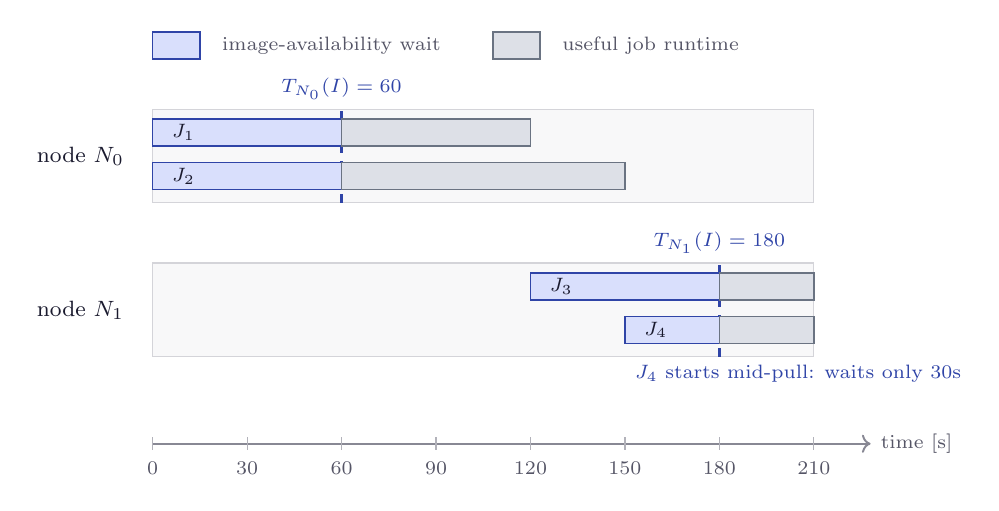
\begin{tikzpicture}[
    x=0.040cm, y=0.85cm,
    lane/.style={draw=SUB!25, fill=SUB!4},
    coldwait/.style={fill=COLD!20, draw=COLD!70!black, line width=0.6pt},
    runtime/.style={fill=RUN!30, draw=RUN!75!black, line width=0.6pt},
    avail/.style={draw=COLD!70!black, dashed, line width=1pt},
    lab/.style={font=\footnotesize, text=INK},
    tick/.style={font=\scriptsize, text=SUB},
    joblabel/.style={font=\scriptsize\bfseries, anchor=west, text=INK},
  ]

  % axis
  \draw[->, SUB!70, line width=0.7pt] (0,0) -- (228,0) node[right, tick] {time [s]};
  \foreach \x in {0,30,60,90,120,150,180,210} {
    \draw[SUB!45] (\x,0.10) -- (\x,-0.10);
    \node[tick, anchor=north] at (\x,-0.12) {\x};
  }

  % node lanes
  \draw[lane] (0,3.6) rectangle (210,5.0);
  \draw[lane] (0,1.3) rectangle (210,2.7);
  \node[lab, anchor=east] at (-6,4.3) {node $N_0$};
  \node[lab, anchor=east] at (-6,2.0) {node $N_1$};

  % availability markers
  \draw[avail] (60,3.6) -- (60,5.0);
  \node[tick, anchor=south, text=COLD!70!black] at (60,5.0) {$T_{N_0}(I)=60$};
  \draw[avail] (180,1.3) -- (180,2.7);
  \node[tick, anchor=south, text=COLD!70!black] at (180,2.7) {$T_{N_1}(I)=180$};

  % N0 jobs
  \draw[coldwait] (0,4.45) rectangle (60,4.85);
  \draw[runtime]  (60,4.45) rectangle (120,4.85);
  \node[joblabel] at (3,4.65) {$J_1$};
  \draw[coldwait] (0,3.80) rectangle (60,4.20);
  \draw[runtime]  (60,3.80) rectangle (150,4.20);
  \node[joblabel] at (3,4.00) {$J_2$};

  % N1 jobs
  \draw[coldwait] (120,2.15) rectangle (180,2.55);
  \draw[runtime]  (180,2.15) rectangle (210,2.55);
  \node[joblabel] at (123,2.35) {$J_3$};
  \draw[coldwait] (150,1.50) rectangle (180,1.90);
  \draw[runtime]  (180,1.50) rectangle (210,1.90);
  \node[joblabel] at (153,1.70) {$J_4$};

  % legend
  \draw[coldwait] (0,5.75) rectangle (15,6.15);
  \node[tick, anchor=west] at (19,5.95) {image-availability wait};
  \draw[runtime] (108,5.75) rectangle (123,6.15);
  \node[tick, anchor=west] at (127,5.95) {useful job runtime};

  % annotation for J4 partial wait
  \node[tick, anchor=west, text=COLD!70!black] at (150,1.05) {$J_4$ starts mid-pull: waits only 30s};

\end{tikzpicture}
\end{document}
